\chapter{Implementació de la Web}

S'ha desenvolupat una web molt senzilla per a tal d'utilitzar aquest recomanador. El recomanador, apart de precís, s'ha de veure si és prou ràpid per a poder donar resultats a una velocitat acceptable pel món web.

La web s'ha desenvolupat mitjançant PHP\footnote{PHP: Hypertext Preprocessor} \cite{php-web}, utilitzant MySQL \cite{mysql-web} per a la base de dades. El motiu per a triar aquest llenguatge ha estat, simplement, que és el llenguatge amb el que més he treballat.

\section{Frontal Web}

El frontal web té les següents parts:

\begin{itemize}
	\item Pàgina principal/cercador (Figura \ref{figure-homepage}).
	\item Resultats de cerca, que és un llistat paginat de resultats (Figura \ref{figure-search-results}).
	\item Detalls d'una pel·lícula i la posibilitat de donar-li una puntuació (Figura \ref{figure-film}).
	\item Login/Registre d'usuari.
\end{itemize}

Adicionalment, un cop t'has registrat i connectat amb el teu compte, tens l'opció d'entrar al recomanador. Aquest mostra un llistat, molt semblant al de resultats de cerca, amb recomanacions per a l'usuari, on les primeres son les que segurament més li interesin, com es pot veure a la figura \ref{figure-recommendations}.

\begin{figure}[h]
  \caption{Pàgina principal.}
  \label{figure-homepage}
  \centering
    
\includegraphics[width=0.5\textwidth]{figs/homepage.png}
\end{figure}

\begin{figure}[h]
  \caption{Pàgina dels resultats de cerca.}
  \label{figure-search-results}
  \centering
    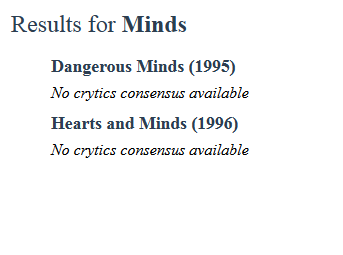
\includegraphics[width=0.5\textwidth]{figs/resultats-busqueda.png}
\end{figure}

\begin{figure}[h]
  \caption{Fitxa d'una pel·lícula.}
  \label{figure-film}
  \centering
    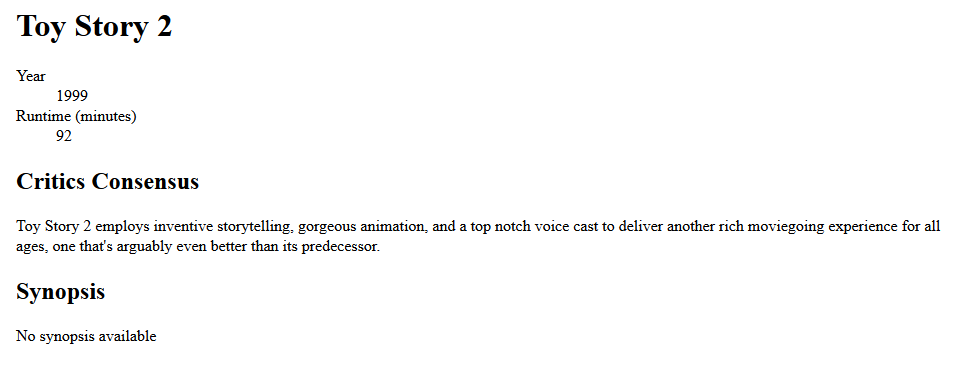
\includegraphics[width=0.85\textwidth]{figs/film.png}
\end{figure}

\begin{figure}[h]
  \caption{Pàgina de recomanació de pel·lícules.}
  \label{figure-recommendations}
  \centering
    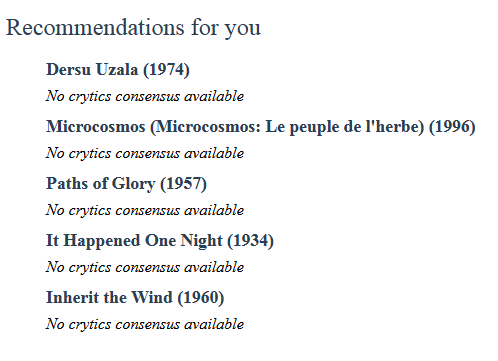
\includegraphics[width=0.5\textwidth]{figs/recommendation.png}
\end{figure}

\section{Zona d'administració}

S'ha realitzat un panell d'administració molt senzill per tal de poder:

\begin{itemize}
	\item Administrar usuaris.
	\item Administrar pel·lícules.
	\item Importar pel·lícules desde \emph{Rotten Tomatoes}.
\end{itemize}

\section{Integració amb el recomanador}

Donat que la pàgina està feta amb PHP i el recomanador en canvi en Java, s'ha hagut de buscar un sistema per a comunicar aquests dos components. El que s'ha acabat utilitzant ha estat Gearman \cite{gearman-web}, el qual és un sistema composat per tres parts que seràn explicades a continuació.

\subsection{Servidor}

El servidor de Gearman és un procés que s'encarrega de rebre les conexions tant dels \emph{treballadors} com dels \emph{clients} i dirigeix la comunicació entre aquests altres dos elements.

\subsection{Treballador}

El treballador és un procés encarregat de dur a terme una o més tasques anomenades \emph{funcions}. Les funcions reben una cadena de bytes d'entrada i el seu retorn es una altra cadena de bytes. A més a més, tenen la possibilitat d'anar enviant els resultats a mesura que els van obtenint, enlloc d'haver de fer esperar al client a que estigui tot calculat per tal d'enviar la resposta.

Al sistema definit el treballador és el codi en Java que s'encarrega de realitzar les recomanacions. Com a entrada rep únicament un nombre, que es l'identificador de l'usuari, i com a sortida retorna una cadena, codificada en JSON\footnote{JavaScript Object Notation} de les recomanacions sol·licitades.

\subsection{Client}

El client és l'element que crida a funcions del treballador. Pot fer-ho de dues formes: o bé esperant a que el treballador de Gearman retorni el resultat o sinó directament fent la petició i seguint amb el procés. Això permet o bé comunicació amb un procés, o l'execució de tasques en segon plà.

A l'aplicació el client és utilitzat per el codi PHP per a obtenir resultats del recomanador.

\section{Configuració del servidor}

Un cop explicades les eines necessàries per a solucionar els diferents problemes que hi havia a l'hora d'integrar el sistema, cal configurar el servidor, que donat que era per a fer proves, era una màquina virtual per a funcionar amb totes les eines necessàries. Aleshores, les eines utilitzades finalment han estat.

\begin{itemize}
	\item{PHP 5.4} per a l'execució del codi.
	\item{MySQL} com a motor de base de dades.
	\item{Apache2} com a servidor HTTP, que deriva les peticions cap a PHP.
	\item{Gearman Server} per a poder comunicar-nos amb el recomanador de forma senzilla.
	\item{Java} per a executar el recomanador.
\end{itemize}

A més, per a PHP calien diversos paquets, per tal de realitzar les diferents tasques.

\begin{itemize}
	\item{APC}: un sistema d'optimització de PHP. Evita que s'hagi de fer el procès de compilació dels fitxers de codi amb cada petició guardant una copia del codi compilat a memòria.
	\item{Gearman} per tal de poder comunicar-se amb el servidor de Gearman per a fer peticions al recomanador.
	\item{cURL} per tal de poder fer peticions a altres webs, en el nostre cas, a la API\footnote{Application Programming Interface} de \emph{Rotten Tomatoes}.
\end{itemize}